
\chapter{Solana}

\begin{wrapfigure}{r}{0.40\textwidth}
    \centering
    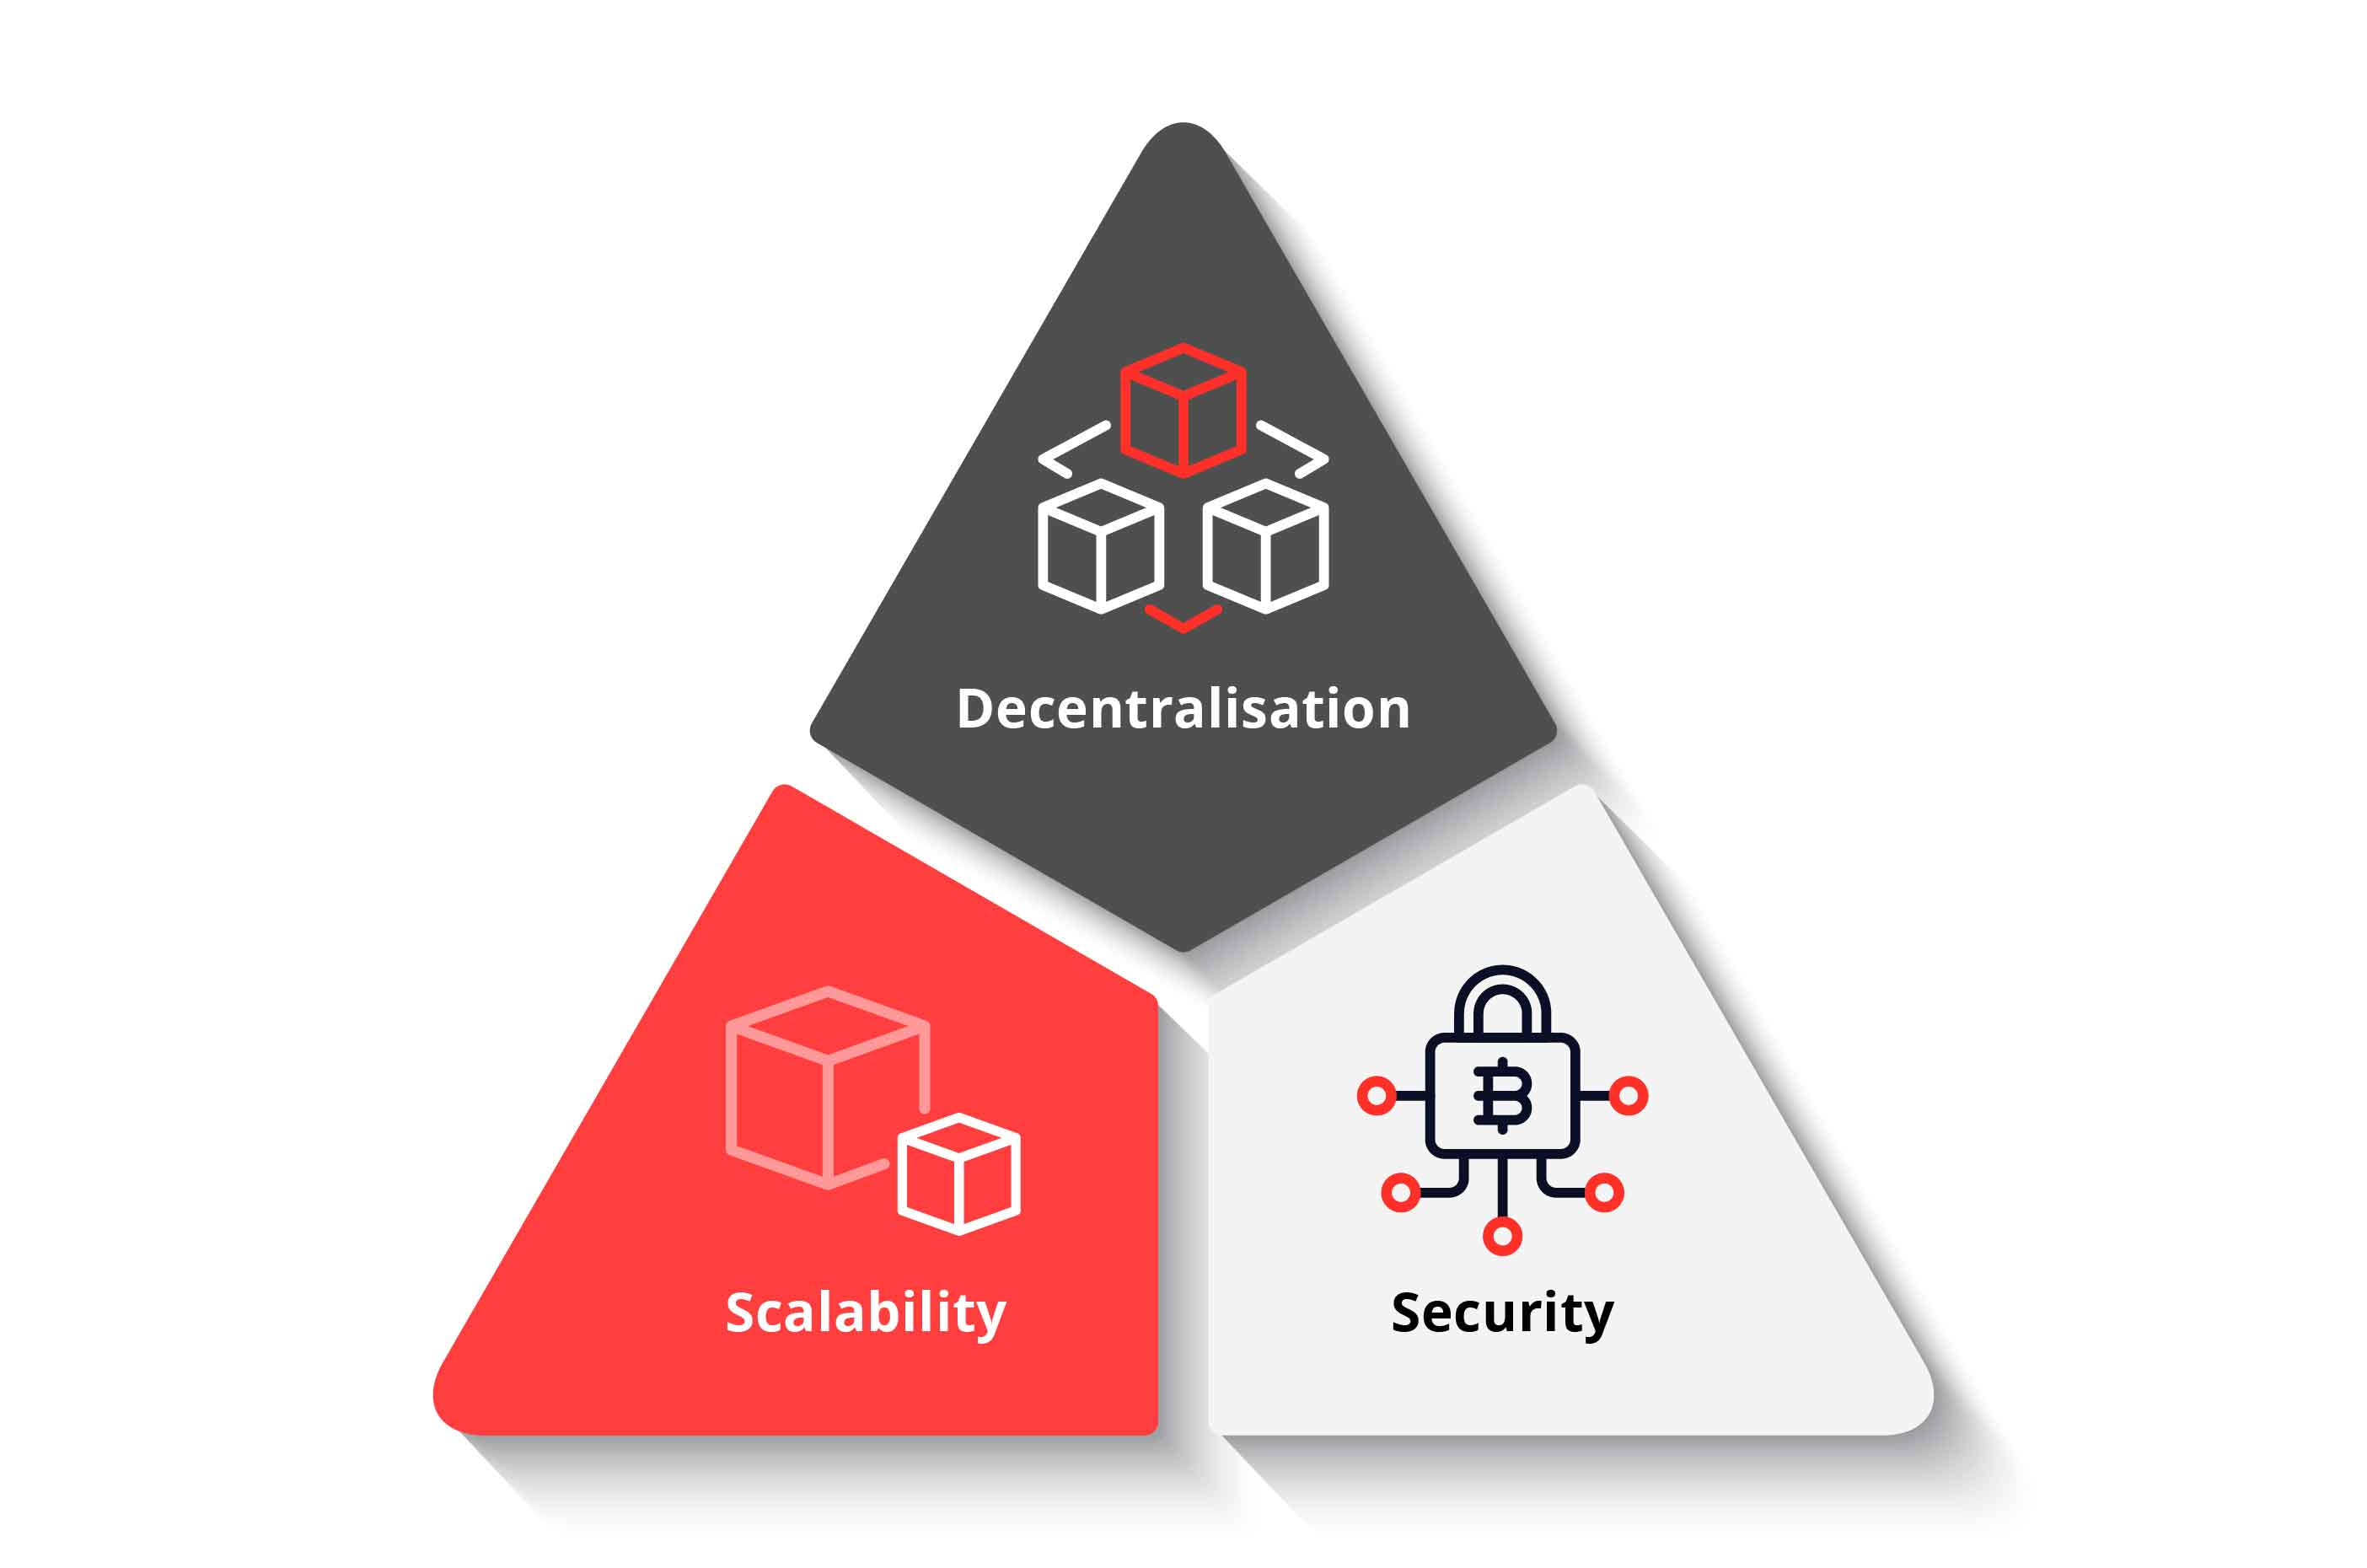
\includegraphics[width=0.40\textwidth]{solana/assets/blockchain-trilemma.png}
    \caption{The blockchain trilemma}
    \label{fig:blockchain-trilemma}
\end{wrapfigure}

Solana seems to be an interesting trade-off choice in the blockchain trilemma when compared to the likes of Ethereum. The blockchain trilemma is a trade-off between decentralization, security and scalability. Solana seems to be focusing more on the scalability, while security and decentralization are arguably worse as compared to Ethereum.

Very briefly, the blockchain trilemma goes as follows:
\begin{itemize}
    \item \textbf{Decentralization}: The more decentralized a blockchain is, the more secure it is. This is because it is harder for a single entity to take over the network. This is often measured using the \textit{nakamoto coefficient}\footnote{\textbf{Nakamoto Coefficient}: First proposed by Balaji Srinavasan and Leland Lee and named in honor of Satoshi Nakamoto, the pseudonymous creator of Bitcoin, the Nakamoto Coefficient is a measure of the smallest number of independent entities that can act collectively to shut down a blockchain. It is often closely related to the "Gini Coefficient" of the economical system under question. For current nakamoto number of public blockchains using Proof-of-Stake, see \href{https://nakaflow.io/}{https://nakaflow.io/}}.
    \item \textbf{Security}: The more secure a blockchain is, the more guarantees it can provide, the harder it becomes for an adversary to compromise the system. Guarantees come in the form of economically-backed guarantees (which are subject to elements such as total tokens staked in a network etc) or mathematically-backed guarantees (such as zk proofs, hash non-collision etc.).
    \item \textbf{Scalability}: The more scalable a blockchain is, the more user requests, often measured in form of "transactions per second" or TPS it can perform.
\end{itemize}

Solana focuses a whole lot more on the "transactions per second" part of the blockchain, a.k.a. the "scalability" aspect.


\section{The Transaction Processing Unit}
\section{Proof of History: VDF based transaction ordering}
\section{Entries, Slots, Bank}